\subsection{Intromolecular}
The interface of the FERM domain and the kinase is of special interest since the domains have to dissociate for a full activation. Therefore contacts and contact areas at the interface are investigated using the following methods.\\
\subsubsection{ConAn}
ConAn is a completely, bug free, user friendly and well documented tool to analyze the distances between all residue pairs in a molecule. It is great, believe me, and totally works out of the box. \textit{Some explanation about Contact maps? But should be self explaining :D}
\subsubsection{Contact area}
The contact area of the interface is determined with the solvent accessible surface area (SASA) and is defined as
\begin{equation}
	\text{CA} = \frac{1}{2} \left(\text{SASA}_\text{FERM} + \text{SASA}_\text{kinase} - \text{SASA}_\text{FERM-kinase}\right)
\end{equation}
The calculation of the SASA values was done with \gromacs{} sasa tool.
\subsection{Intermolecular}
In order to determine the cluster behaviour of FAK intermolecular contacts of FAK molecules have to be considered. For this purpose, the following terms are defined.
\paragraph{Interaction} Proteins or parts of proteins interact, if their minimal distance is smaller than a cut-off distance (here $1.5\,\si{\nano\metre}$).
\paragraph{Neighbour} Protein A is a neighbour of Protein B, if they are interacting. One protein can have several neighbours. For a more detailed characterisation the following types are defined (see also \autoref{methods:inttypes}):
\begin{enumerate}[label={type \theenumi:}, leftmargin=*]
	\item only the FERM domain interacts with only the FERM domain of the other protein
	\item only the kinase interacts with only the kinase of the other protein
	\item only the FERM domain interacts with only the kinase of the other protein
	\item the FERM domain is interacting with both, the FERM and kinase of the other protein
	\item the kinase is interacting with both, the FERM and kinase of the other protein
	\item the FERM domain is interacting with the FERM domain of the other protein and the kinase is interacting with the kinase of the other protein
	\item the FERM domain is interacting with the kinase of the other protein and the kinase is interacting with the FERM domain of the other protein
\end{enumerate}
\paragraph{Cluster} Protein A belongs to a cluster, if it has at least one neighbour inside the cluster. Two neighbouring proteins form a cluster of size 2. One protein can only belong to one cluster.
%
%
%
\begin{figure}
	\centering
	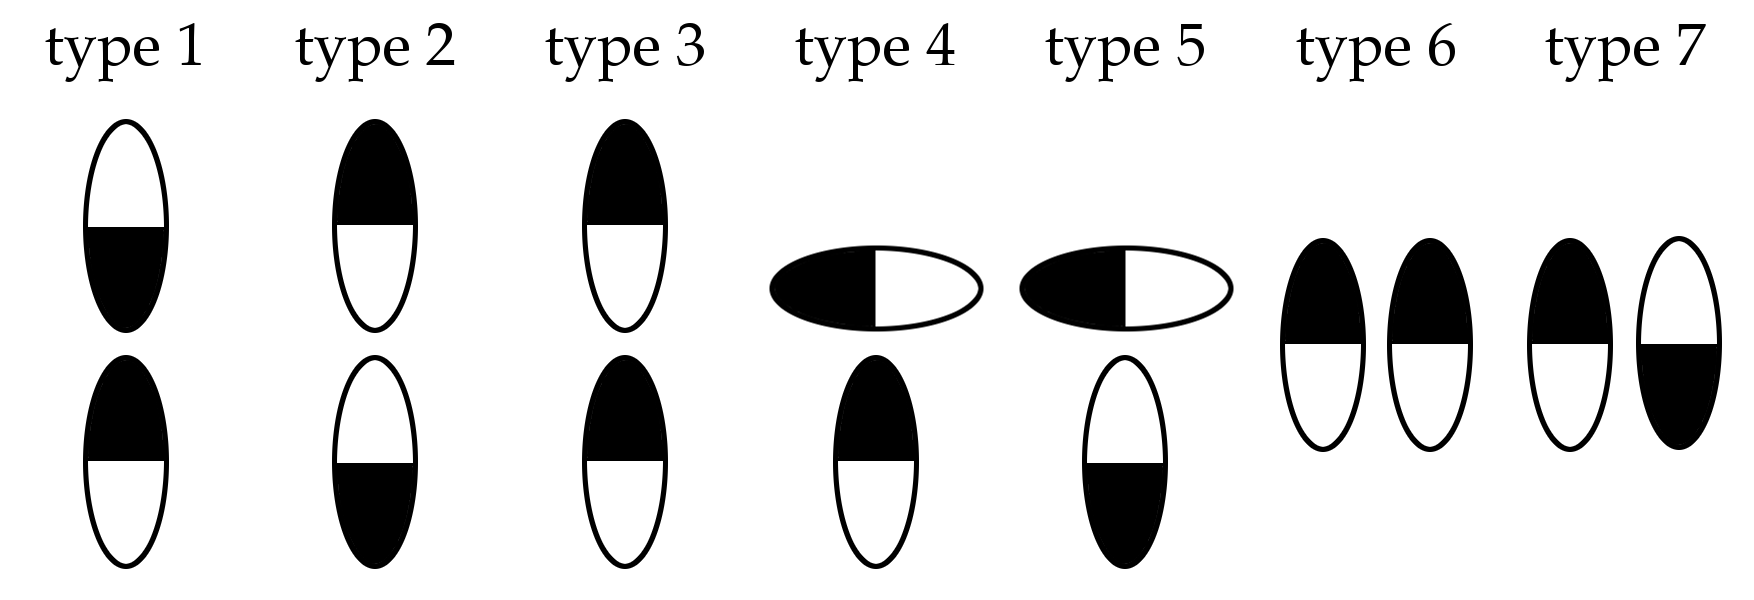
\includegraphics[width=\textwidth]{figures/introduction/classification}
	\captionof{figure}{Different interaction types for two FAK molecules}
	\label{methods:inttypes}
\end{figure}
%
%
%